%!TEX root = ../../thesis.tex

The non-\WW diboson background comprises the \Wgamma, \Wgstar, \WZ and \ZZ processes (in 
order of contribution to the signal region). \Wgamma events feature a prompt photon that 
passes the electron selection, via an asymmetric conversion (\epluseminus production). The 
other processes have signatures of \HepProcess{\Plepton\Pnu\Plepton\Plepton}, 
\HepProcess{\Plepton\Plepton\Plepton\Plepton} or \HepProcess{\Plepton\Plepton\Pnu\Pnu}, and 
usually contribute when one or more leptons fail object selection (\eg 
\unit{$\pt < 10$}{\GeV} or $\mods{\eta} > 2.5$).



\subsection{Same-sign control region}
\label{sec:diboson:sscr}

In non-\WW diboson backgrounds, a symmetry is expected to exist between opposite-sign (OS) 
and same-sign (SS) dilepton events; this is particularly true in the \emch/\mech channels, 
where asymmetric final states are removed. Conversely, the \WW, top and \DY backgrounds 
only contribute to the OS sample. Finally, the \Wjets background displays a partial OS/SS 
symmetry, as described in \Section~\ref{sec:wjets:wjet_bkg}. Thus, SS events can be used to 
estimate the non-\WW diboson background in the OS signal region, whilst validating the 
\Wjets estimation.

An SS control region (CR) is defined using identical criteria to the OS signal region (SR). 
In the language of \Section~\ref{sec:wjets}, the SS CR events are in the SR of the 
$\mathcal{N}_{\id{\Plepton}\id{\Plepton}\text{,SS}}$ sample. This is used to determine the 
normalisation of the non-\WW diboson background, whilst the shapes of observables used in 
the fitting procedure (\ie \mt, \mll and \ptsubleadlep) are modelled by MC. This is 
equivalent to
\begin{equation}
	N_{\HepProcess{\PV\PV}}^{\text{pred,SR}} &= \alpha_{\HepProcess{\PV\PV}} \cdot \parenths{N^{\text{data,CR}} - N_{\text{non-}\HepProcess{\PV\PV}}^{\text{pred,CR}}} \label{eq:sscr} \\
	\alpha_{\HepProcess{\PV\PV}} &= N_{\HepProcess{\PV\PV}}^{\text{MC,SR}} / N_{\HepProcess{\PV\PV}}^{\text{MC,CR}}
\end{equation}
where $\HepProcess{\PV\PV} = \Wgamma + \Wgstar + \WZ + \ZZ$ and 
$N_{\text{non-}\HepProcess{\PV\PV}}^{\text{pred,CR}}$ is dominated by \Wjets. The 
extrapolation $\alpha_{\HepProcess{\PV\PV}}$ represents the MC predictions for shapes of
observables, since the OS/SS symmetry implies that the total normalisation is unchanged. 

The SS CR method is only used in the 0-jet and 1-jet bins of the \emch/\mech channels, 
using a combined \emch{}+\mech channel to define the CR. All other signal regions use 
estimate the non-\WW diboson background using MC only.

Uncertainties in the normalisation of the constituent processes will cancel if the 
composition of the non-\WW diboson background is the same in SS and OS events; this is 
modelled by MC. However, uncertainties in the shapes of distributions remain, since these 
are not constrained by the SS CR method. Additionally, the uncertainty component of the OS 
\Wjets background that is correlated between OS and SS will cancel in the SS CR method; an 
increase in the SS \Wjets background will be compensated by a decrease in the non-\WW 
diboson background, and vice versa.

To estimate the non-\WW diboson background in regions other than the SR, the method is 
viewed as providing a simple data-driven normalisation factor. This is equivalent to 
neglecting the extrapolation uncertainties, but is helpful when plotting observables. The 
normalisation factors are measured to be \stat{0.96}{0.07} in the 0-jet bin and 
\stat{0.93}{0.13} in the 1-jet bin\todo{update}. 

\Figure~\ref{fig:sscr} validates the MC shape modelling of the fit observables in the SS 
CRs, following application of the normalisation factors. Good agreement with experimental 
data is observed. Note that these SS distributions are not directly used, since only the 
total number of events in the SS CRs are used in (\ref{eq:sscr}).

\begin{figure}[p]
	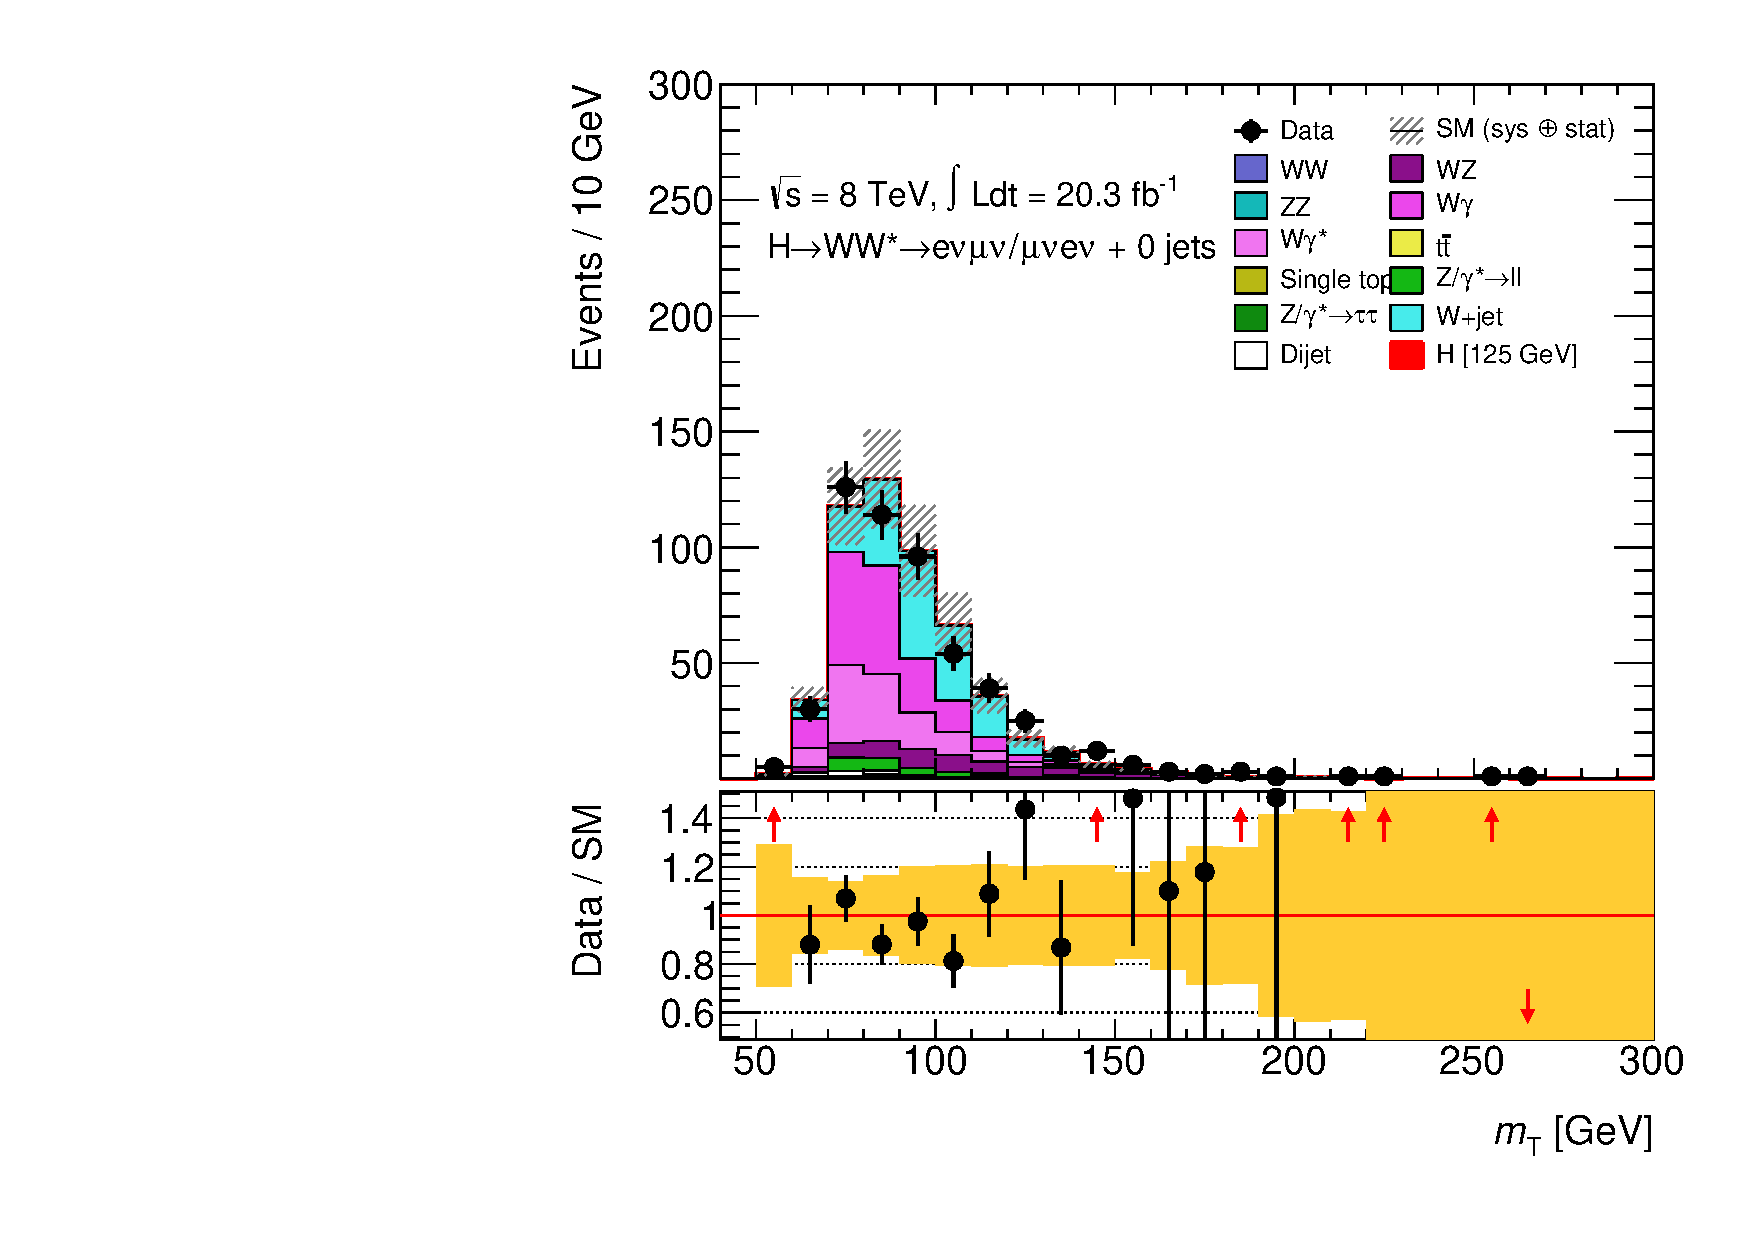
\includegraphics[width=0.48\textwidth]{tex/backgrounds/emme_CutFRecoil_0jet_sscr_MT_TrackHWW_Clj_mh125_lin}
	\hfill
	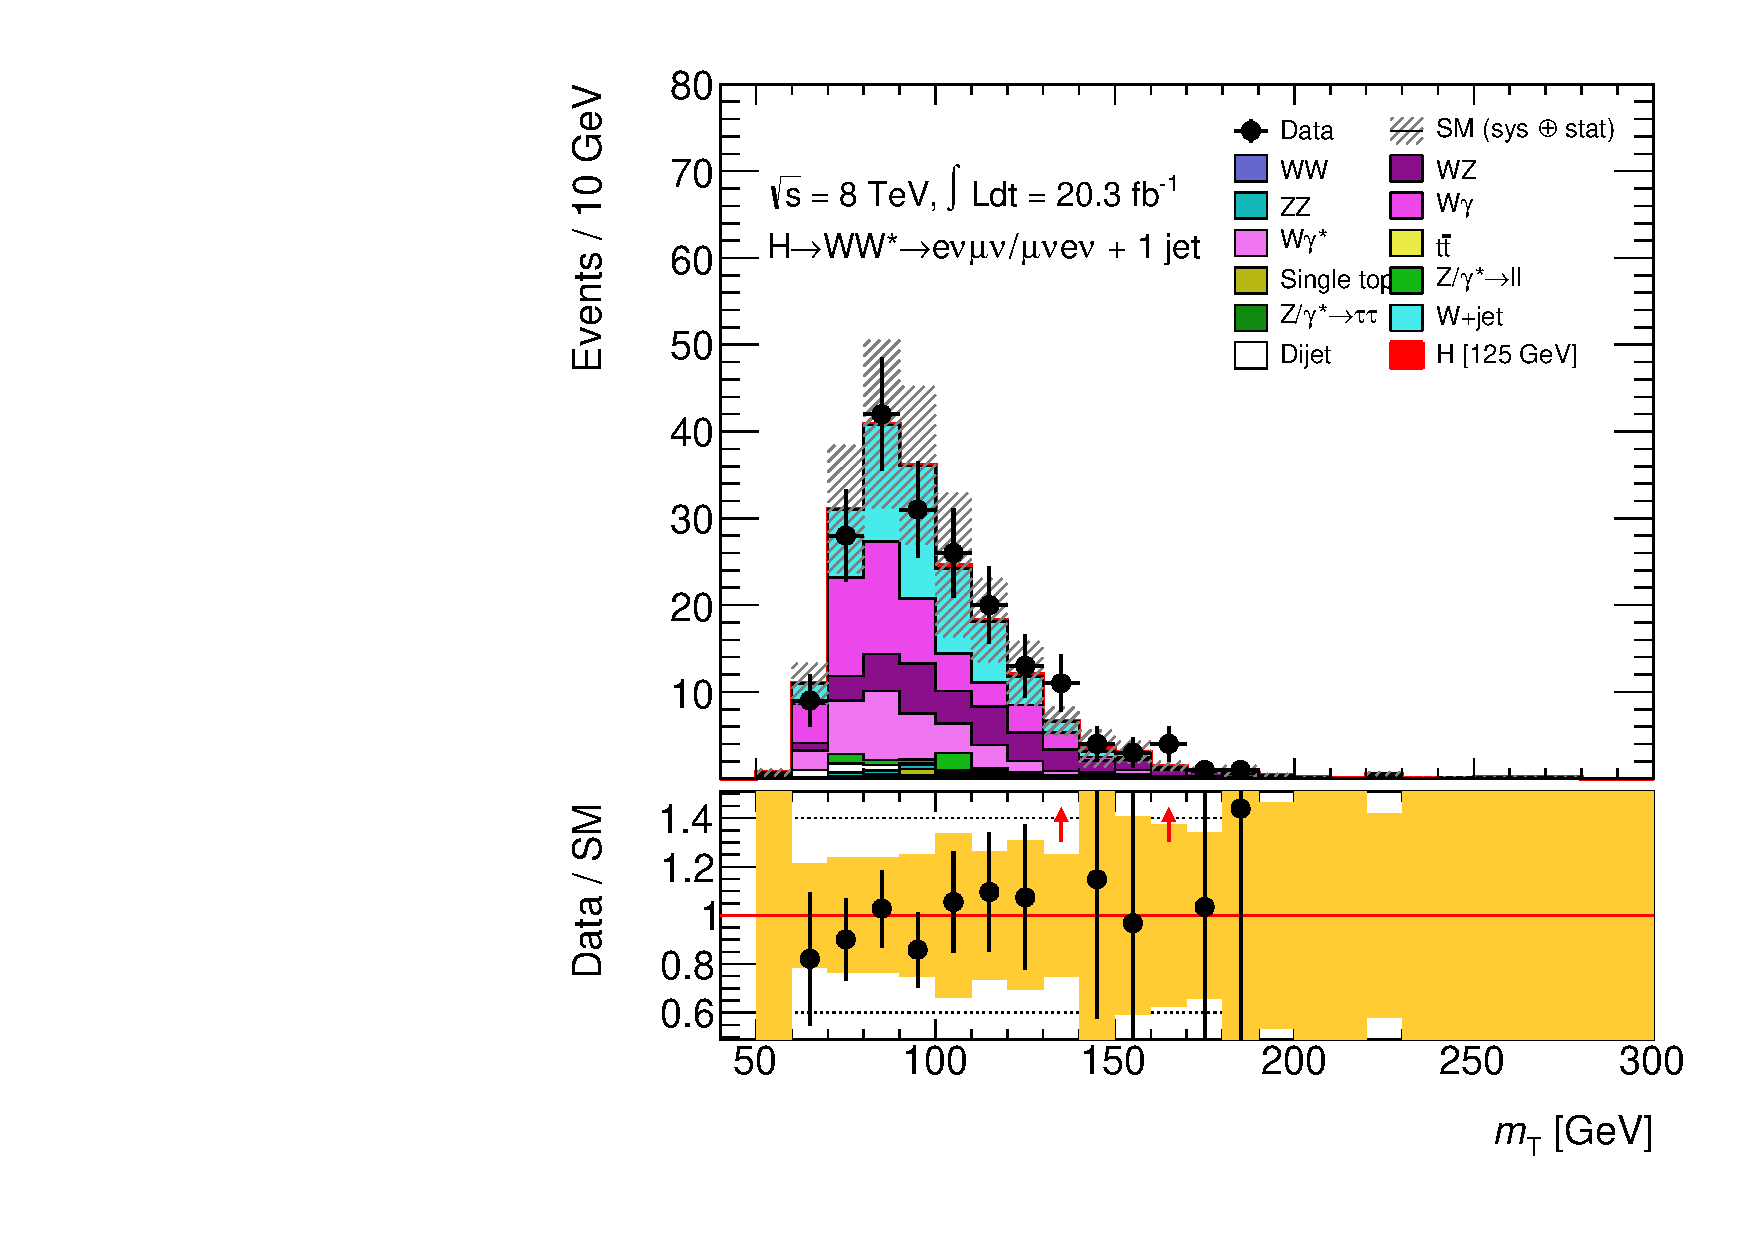
\includegraphics[width=0.48\textwidth]{tex/backgrounds/emme_CutFRecoil_1jet_sscr_MT_TrackHWW_Clj_mh125_lin}
	\\
	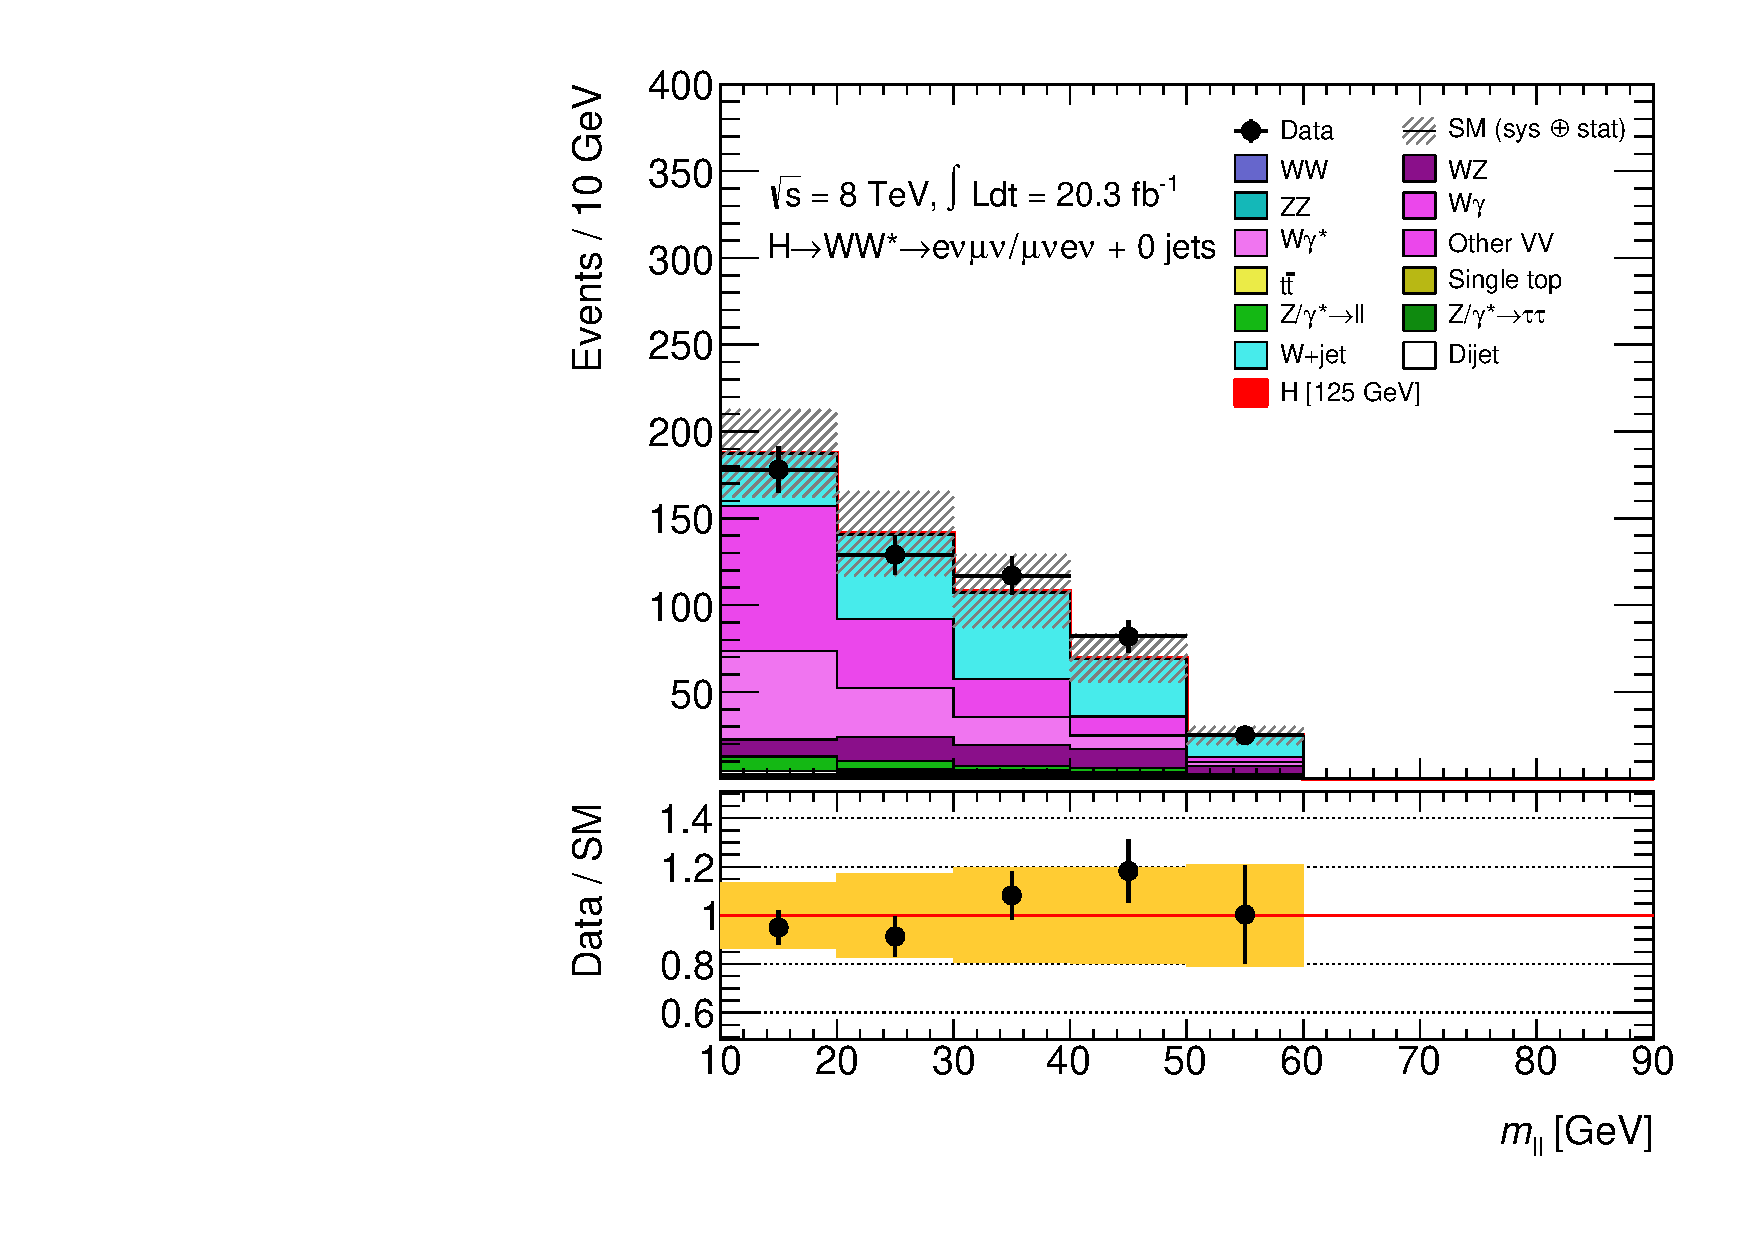
\includegraphics[width=0.48\textwidth]{tex/backgrounds/emme_CutFRecoil_0jet_sscr_Mll_zoom_mh125_lin}
	\hfill
	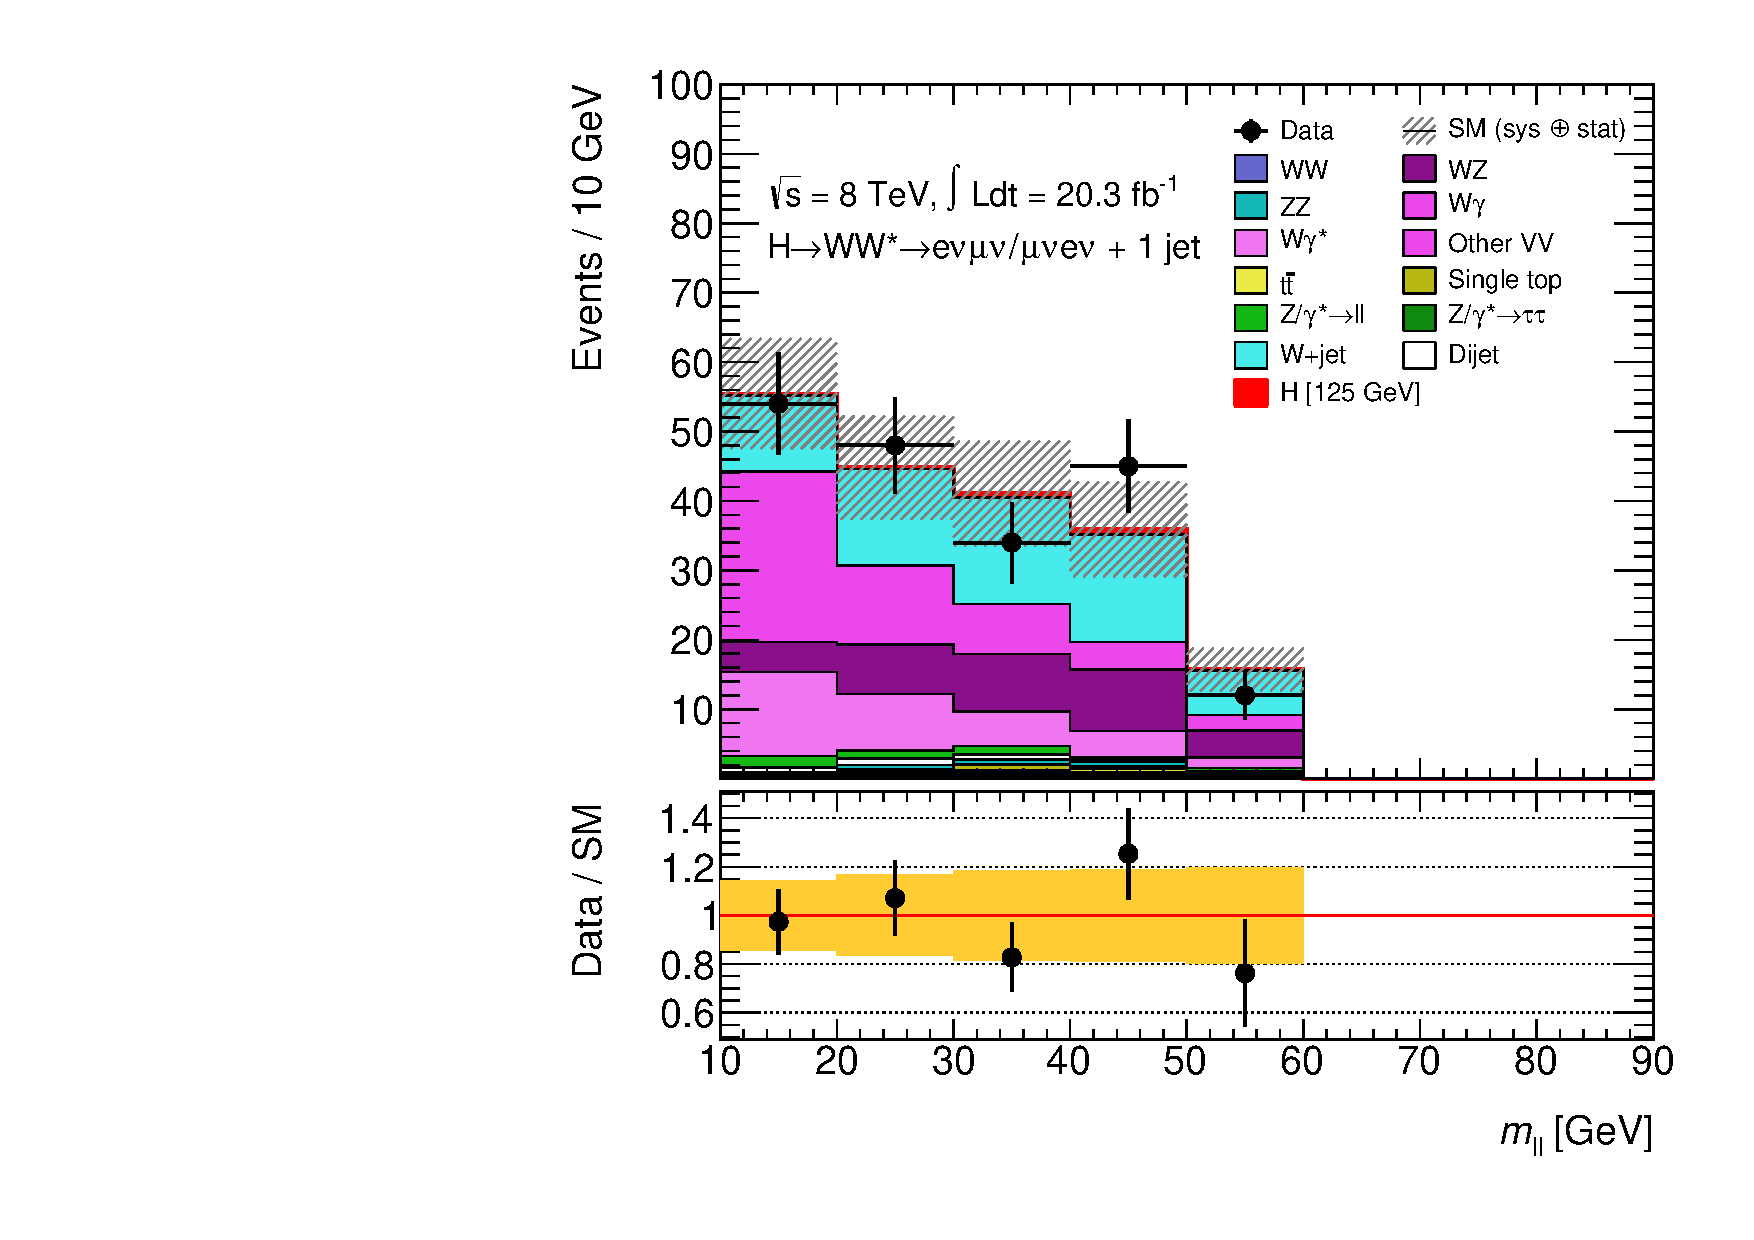
\includegraphics[width=0.48\textwidth]{tex/backgrounds/emme_CutFRecoil_1jet_sscr_Mll_zoom_mh125_lin}
	\\
	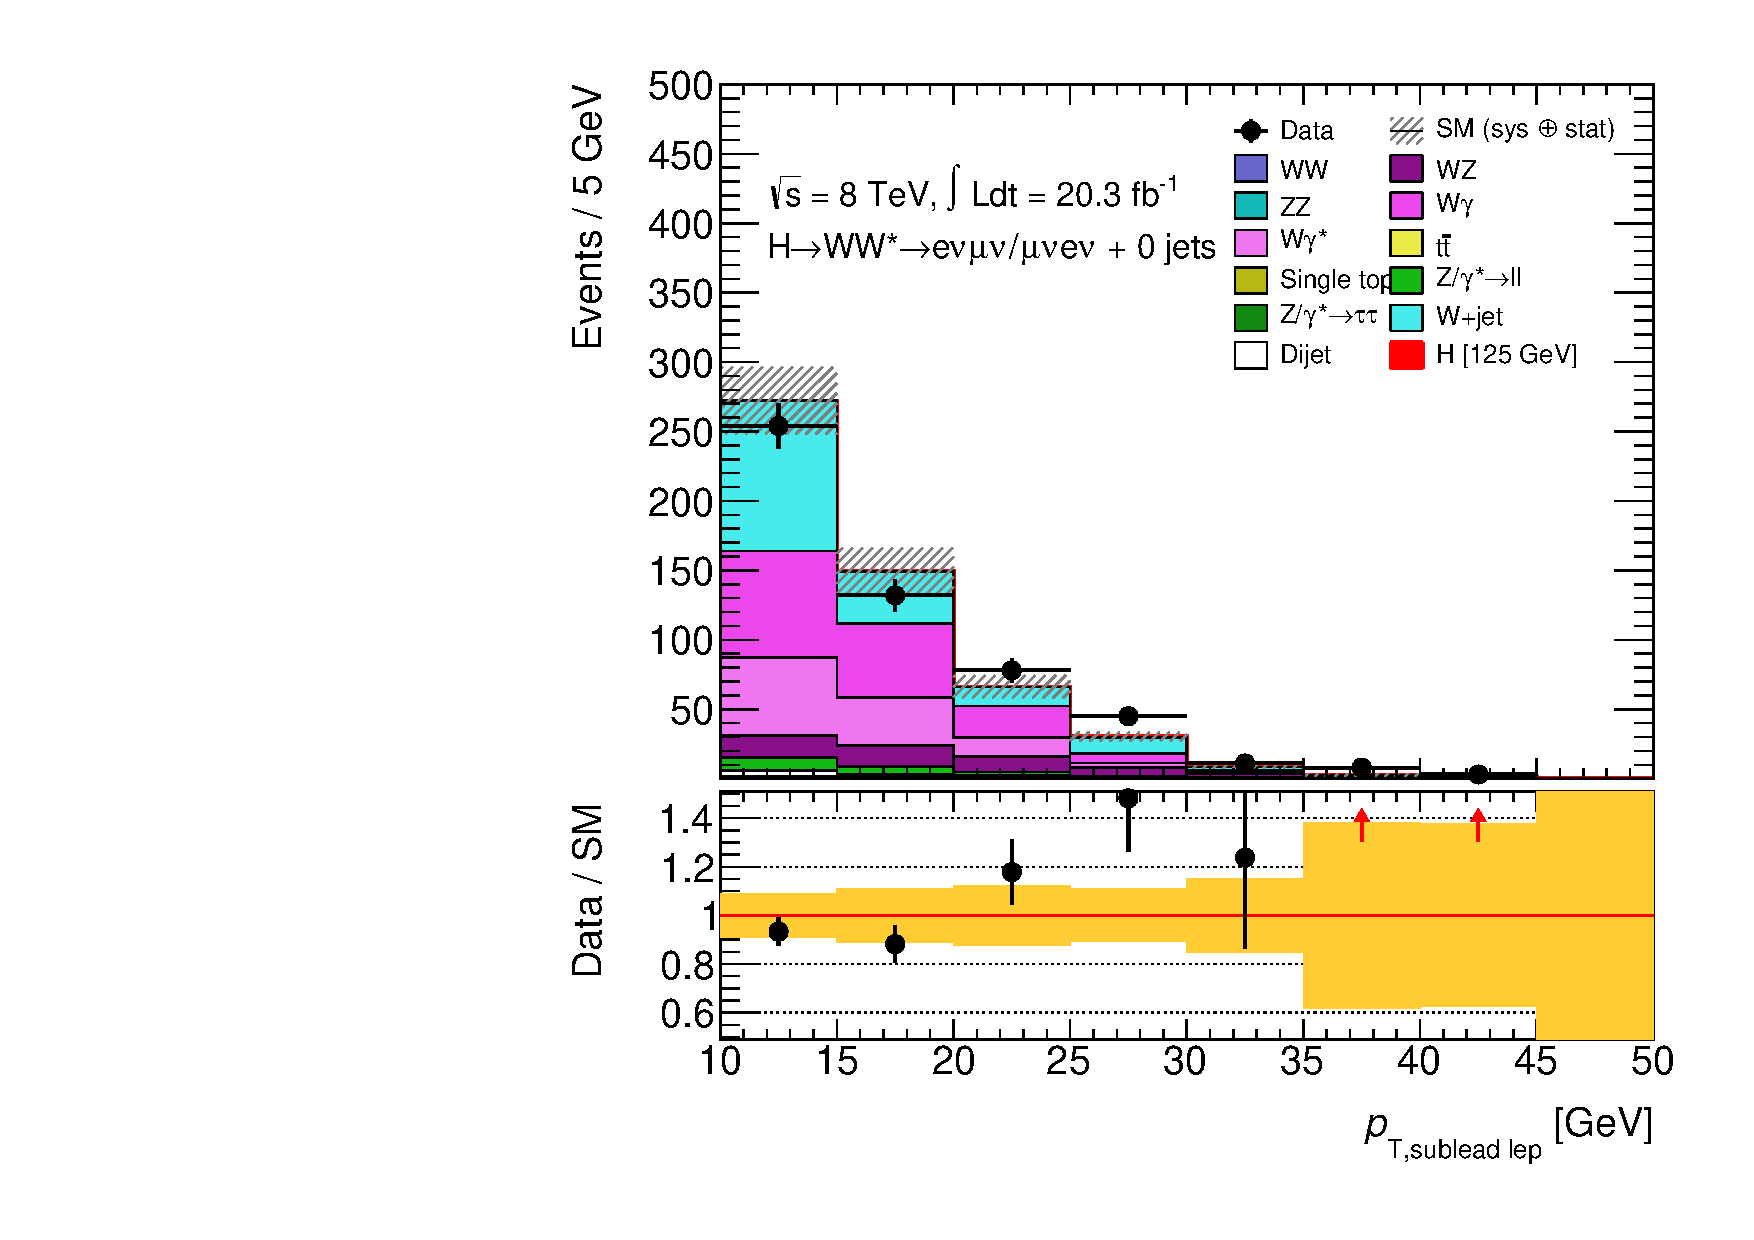
\includegraphics[width=0.48\textwidth]{tex/backgrounds/emme_CutFRecoil_0jet_sscr_lepPtSubLead_zoom_mh125_lin}
	\hfill
	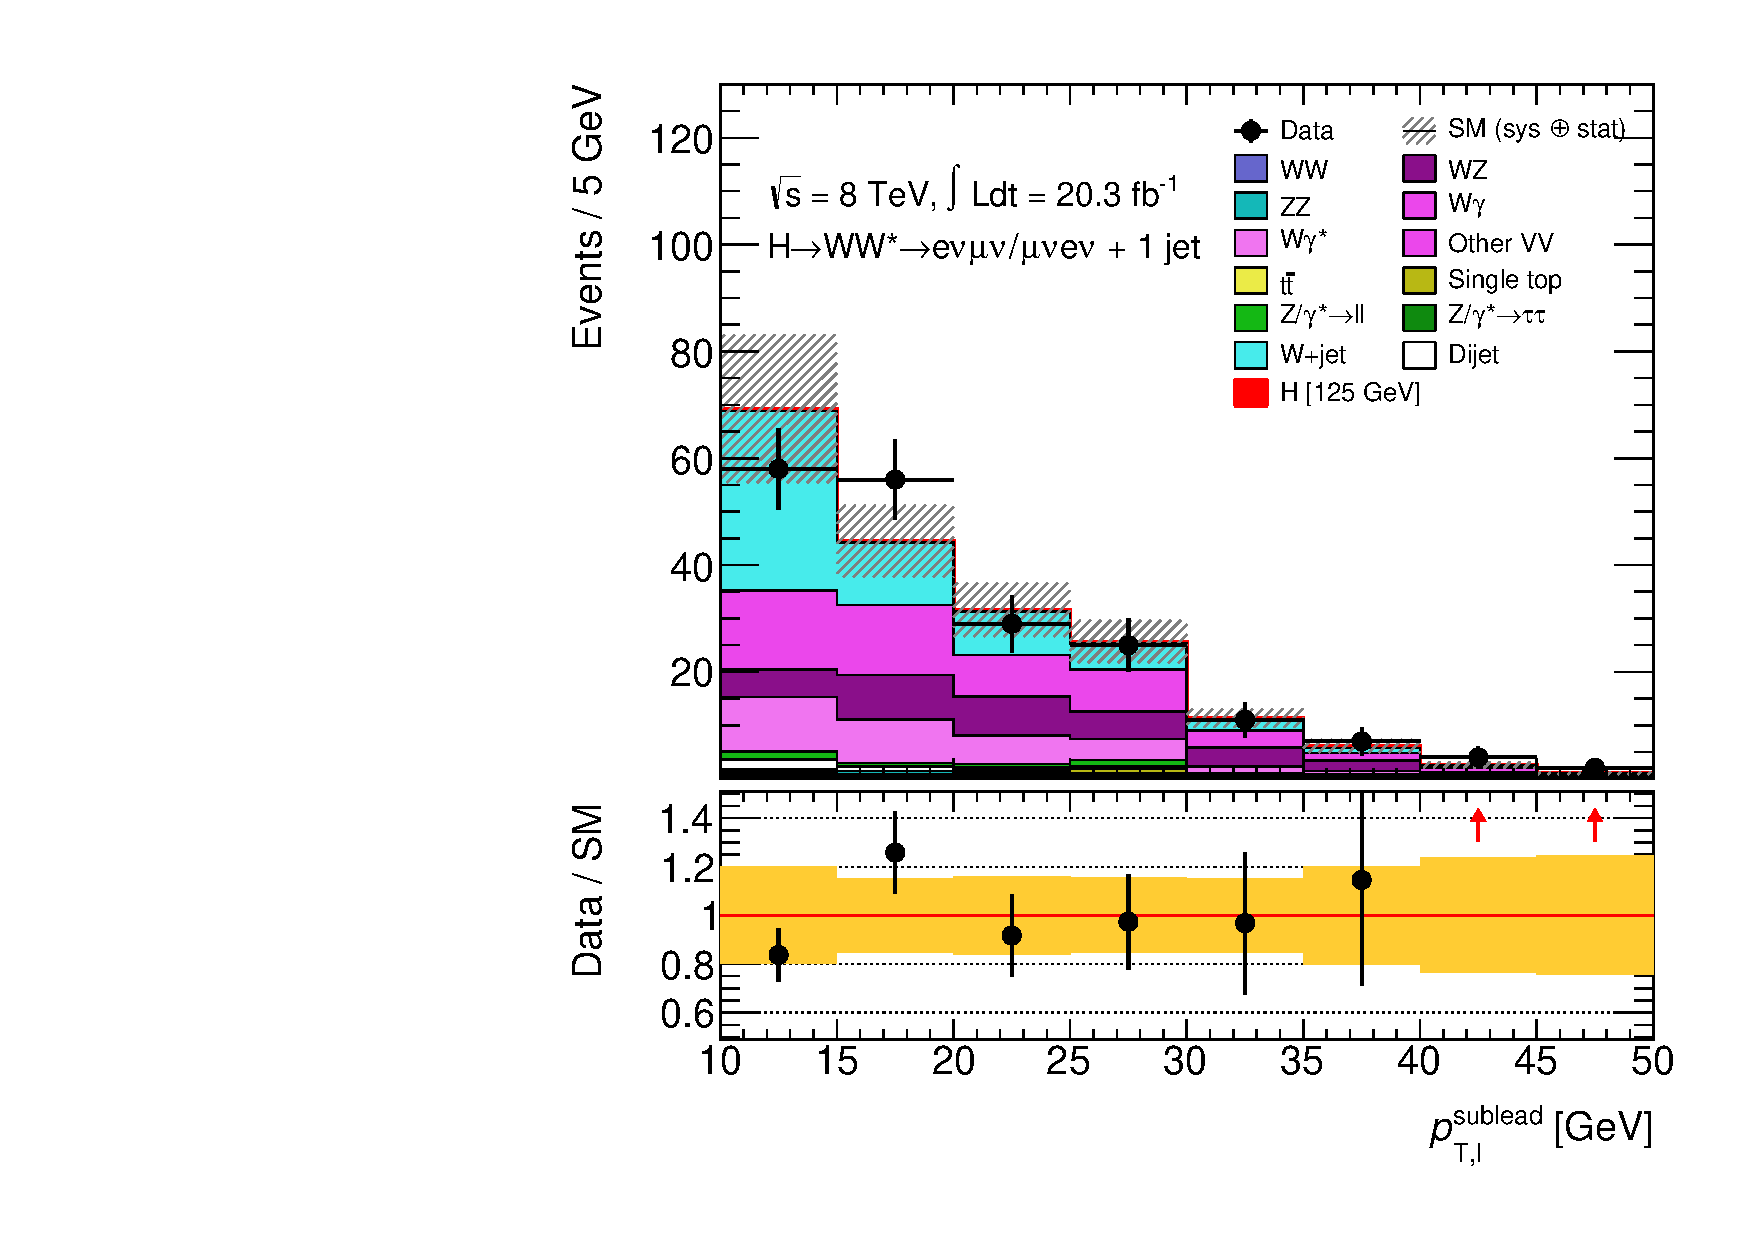
\includegraphics[width=0.48\textwidth]{tex/backgrounds/emme_CutFRecoil_1jet_sscr_lepPtSubLead_zoom_mh125_lin}
	\caption{The \mt (top), \mll (middle) and \ptsubleadlep (bottom) distributions in the 
	0-jet (left) and 1-jet (right) same-sign control regions. Normalisation factors are 
	applied.}
	\label{fig:sscr}
\end{figure}



\subsection{\Wgamma}
\label{sec:diboson:wgamma}

\Wgamma events enter the dilepton sample when the photon fakes an electron. This is usually 
caused by an asymmetric \HepProcess{\Pphoton \HepTo \epluseminus} conversion, where only 
one electron passes the object selection. This background is suppressed by the electron 
identification criteria, which require a hit in the first pixel layer and no conversion 
vertex (see \Section~\ref{sec:objects:electrons}).

\Wgamma is modelled by \meps{\alpgen}{\fherwig} and normalised to the NLO cross section 
calculated with \mcfm. Modelling is tested with a SS dilepton sample of \emch/\mech events, 
but where the electron object is required to have a conversion vertex and no hit in the 
first pixel layer (\ie the photon conversion rejection criteria are inverted). Validation 
regions (VRs) are defined in the 0-jet and 1-jet bins, using the corresponding signal 
region cuts. Experimental data are well described, as seen in \Figure~\ref{fig:wgamma:vr}.

\begin{figure}[t]
	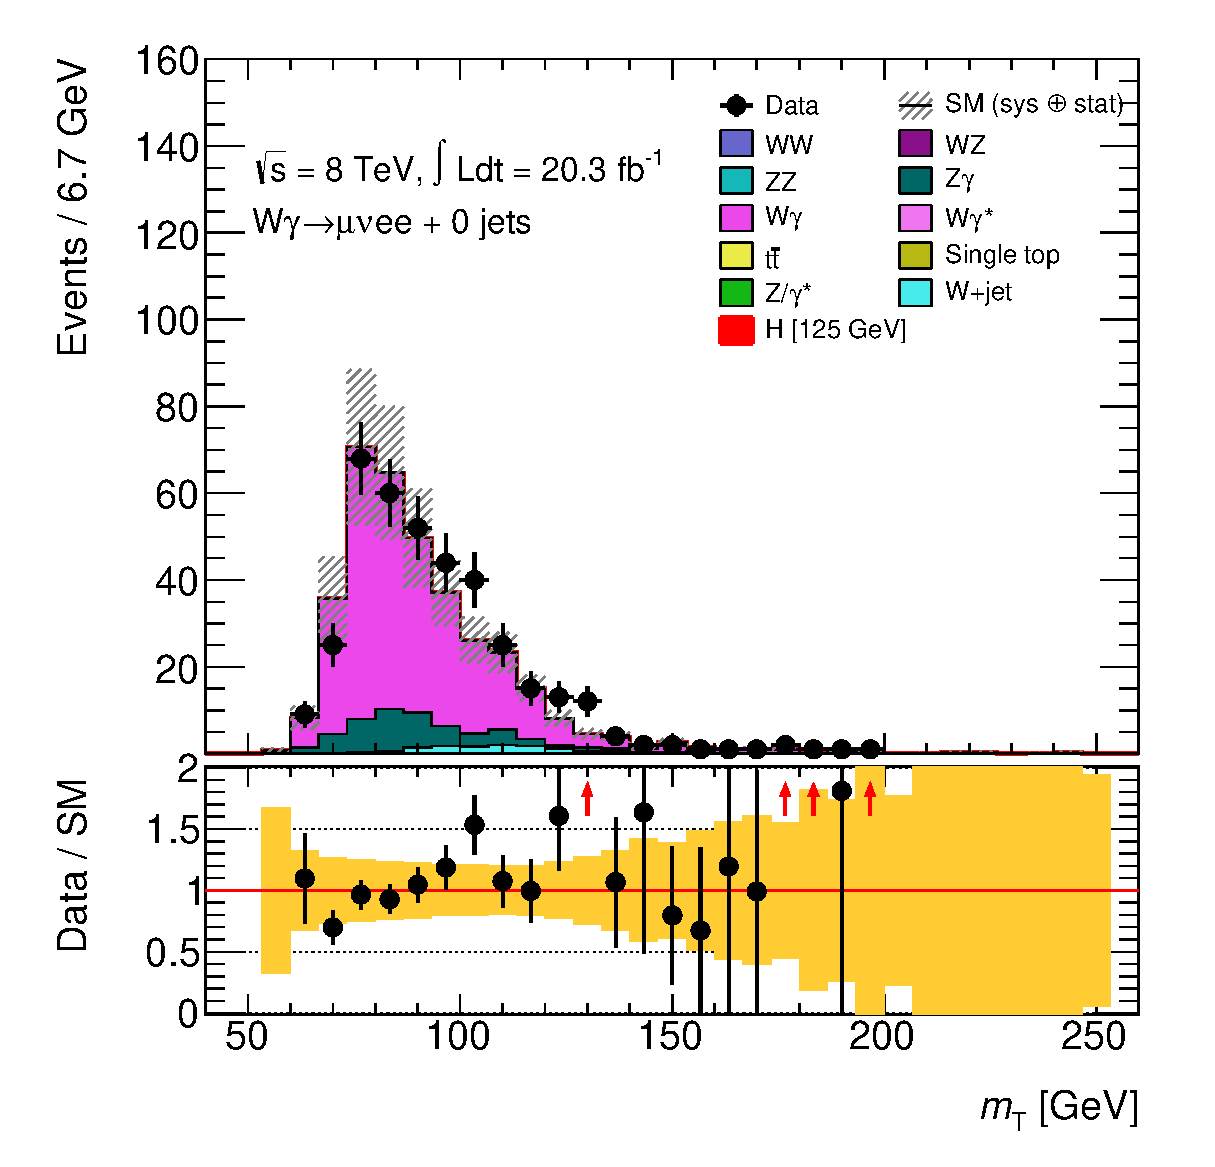
\includegraphics[width=0.48\textwidth]{tex/backgrounds/Wgamma/CutTopoDPhill_0jet_MT_TrackHWW_Clj_mh125_lin}
	\hfill
	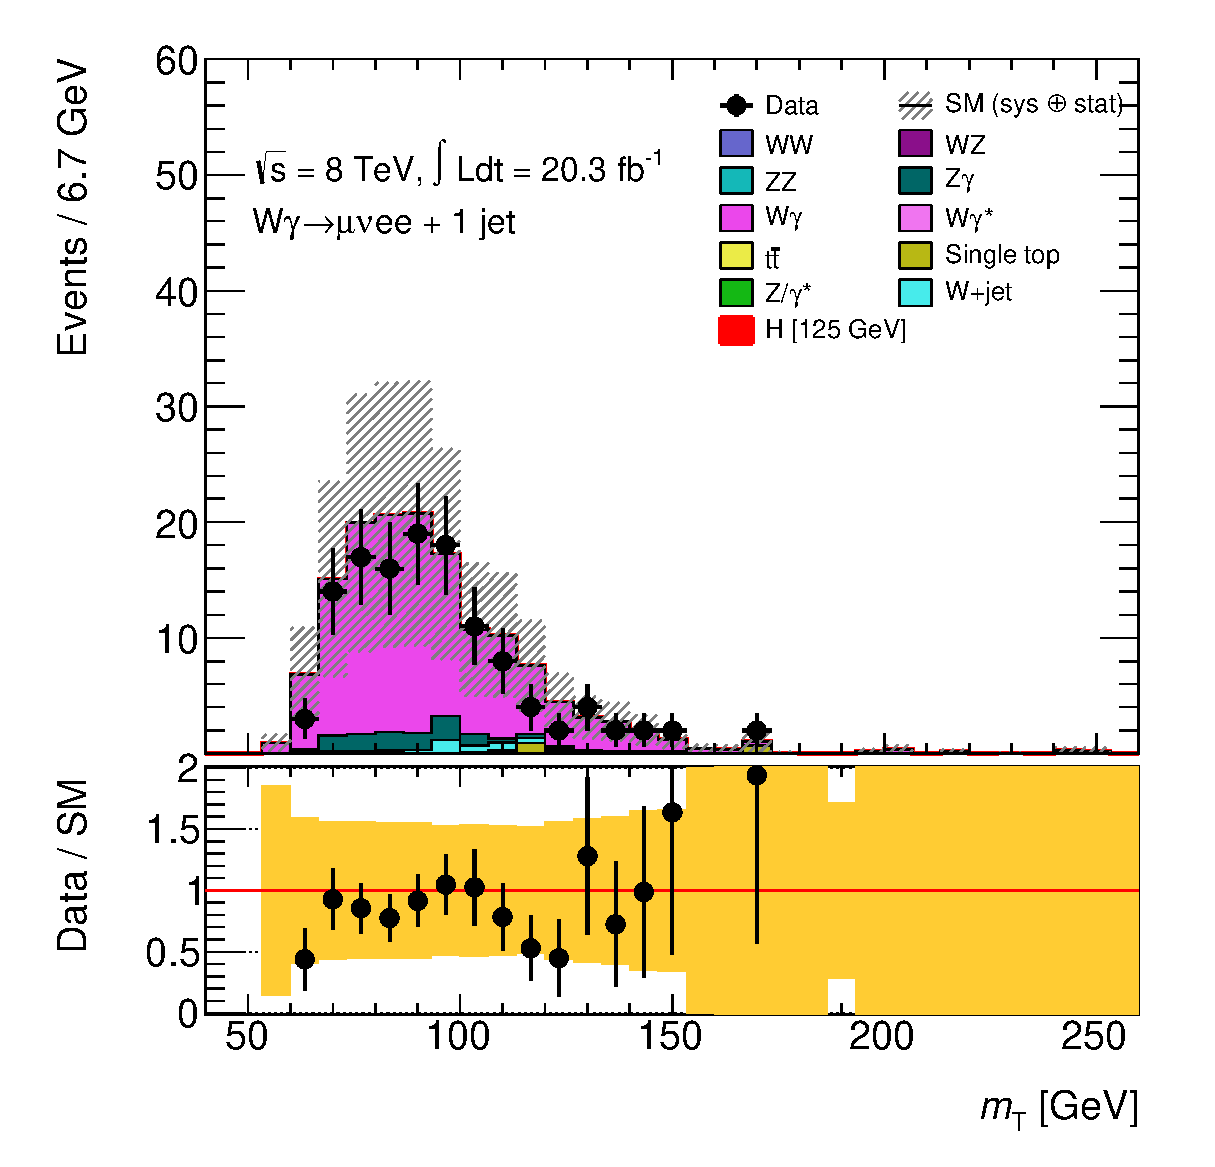
\includegraphics[width=0.48\textwidth]{tex/backgrounds/Wgamma/CutTopoDPhill_1jet_MT_TrackHWW_Clj_mh125_lin}
	\caption{The \mt distribution in the 0-jet (left) and 1-jet (right) \Wgamma validation 
	regions. The shaded error band includes statistical and theoretical uncertainties, in 
	addition to those associated with conversion modelling.}
	\label{fig:wgamma:vr}
\end{figure}

As the conversion and pixel hit criteria are inverted in the VR, their SR modelling is not 
tested in \Figure~\ref{fig:wgamma:vr}. Unfortunately, it is not possible to define a 
high-purity \Wgamma VR when including these criteria. Instead, 
a \HepProcess{\Zgamma \HepTo \Pmu\Pmu\Pphoton} VR is used to test this modelling. 
Events are selected with an OS muon pair with \unit{$p_{\text{T,\Pmu}}^{\text{lead}} > 
22$}{\GeV} and \unit{$p_{\text{T,\Pmu}}^{\text{sublead}} > 10$}{\GeV}, and an additional 
electron with \unit{$p_{\text{T,\Pe}} > 10$}{\GeV}. Low mass resonances are vetoed by 
\unit{$m_{\HepProcess{\Pmu\Pmu}} > 12$}{\GeV}, and events featuring QED FSR are selected by 
\unit{$\mods{m_{\HepProcess{\Pmu\Pmu\Pe}} - \mZ} < 15$}{\GeV}. The selected events are 
\about60\% \Zgamma and \about40\% \Zgstar. The mismodelling is found to depend upon 
$p_{\text{T,\Pe}}$ and so a conversion systematic uncertainty is derived: 25\% for 
\unit{10 -- 15}{\GeV}, 18\% for \unit{15 -- 20}{\GeV} and 5\% for \unit{$>\!20$}{\GeV}.



\subsection{\WZ and \Wgstar}
\label{sec:diboson:wgstar}

Both the \WZ and \Wgstar processes result in a \HepProcess{\Plepton\Pnu\Plepton'\Plepton'} 
final state, peaking in $m_{\HepProcess{\Plepton'\Plepton'}}$ at \mZ and 
$2m_{\Plepton'}$ respectively (due to the different \PZ and \Pphoton propagators). Their 
interference at intermediate $m_{\HepProcess{\Plepton'\Plepton'}}$ is non-negligible, and 
so these processes are generated together.

It is technically difficult to generate MC events with very low 
$m_{\HepProcess{\Plepton'\Plepton'}}$. For this reason, the phase space is generated in two 
parts: high mass ``\WZ'' events with \unit{$m_{\HepProcess{\Plepton'\Plepton'}} > 7$}{\GeV} 
and low mass ``\Wgstar'' events with 
\unit{$m_{\HepProcess{\Plepton'\Plepton'}} < 7$}{\GeV}.\footnote{
	It is these ``\WZ'' and ``\Wgstar''	MC samples that are referred to as the \WZ and 
	\Wgstar backgrounds, though each sample contains both the \WZ and \Wgstar processes.
}
In ambiguous cases ($\Plepton = \Plepton'$), the lowest mass opposite-sign same-flavour 
dilepton pair is used to split the phase space. \WZ is modelled at NLO by 
\meps{\powhegbox}{\pythia{8}}.

\Wgstar is technically difficult to model because it involves integrating over a phase 
space with extremely low mass; the threshold for production is 
$m_{\HepProcess{\Plepton'\Plepton'}} = 2m_{\Plepton'}$, which is \unit{1.022}{\MeV} for 
\HepProcess{\Plepton\Pnu\Pe\Pe}. In previous analysis iterations, \Wgstar was modelled by 
\meps{\madgraph}{\pythia{6}} \cite{HWW-Moriond}. However, this implementation failed to 
produce gauge-invariant results when $m_{\HepProcess{\Plepton'\Plepton'}} \ll \Gamma_{\PW}$ 
\cite{MadGraph:Wgstar}, yielding wildly unphysical events in this region of phase space 
(\eg leptons with \unit{\pt~\about~1}{\TeV}). In an attempt to resolve this problem, events 
with \unit{$m_{\HepProcess{\Plepton'\Plepton'}} < 3$}{\MeV} were removed from the MC 
sample, and events with \unit{3}{\MeV} $< m_{\HepProcess{\Plepton'\Plepton'}} <$ 
\unit{10}{\MeV} were reweighted in order to recover the cross section. Even with this fix, 
this background was associated with a modelling uncertainty of 40\% (evaluated by comparing 
to \sherpa).

\sherpa can produce gauge-invariant results for the full mass range, since it employs a 
complex mass scheme \cite{Sherpa:Wgstar}. A simple LO \sherpa sample underestimates the FSR 
phase space with $p_{\text{T,\HepProcess{\Plepton'\Plepton'}}} > \mW/2$. For this reason, 
\Wgstar is modelled by ME-PS merging with up to one additional parton (see 
\Section~\ref{sec:mc:merging}). It is technically not possible to include further partons 
in the ME-PS merging over the full mass range.

The \sherpa sample is normalised using an NLO $K$-factor of $0.94\pm0.07\,\text{(scale)}$, 
calculated with \mcfm. Due to technical limitations, this is calculated in a high mass 
region \unit{$m_{\HepProcess{\Plepton'\Plepton'}} \in \hardrange{0.5,7}$}{\GeV} and then 
extrapolated down in mass. It is calculated with the \unit{$\ptleadlep > 22$}{\GeV} and 
\unit{$\ptsubleadlep > 10$}{\GeV} criteria.

Since the \Wgstar acceptance of the lepton \pt criteria is strongly related to \njets and 
because the \HWW analysis itself is jet binned, the jet multiplicity distribution must be 
well modelled. For this reason, the \njets distribution is reweighted to that of a \sherpa 
ME-PS merged sample with up to two additional partons, using corrections of 
$0.91\pm0.06\,\text{(scale)}$ in the 0-jet bin, $1.09\pm0.33\,\text{(scale)}$ in the 1-jet 
bin, and $2.0\pm0.5\,\text{(scale)}$ in the \twojet bin. Again, due to technical 
limitations, this was calculated in a high mass region 
\unit{$m_{\HepProcess{\Plepton'\Plepton'}} \in \hardrange{0.5,7}$}{\GeV} and then 
extrapolated down in mass. It was also calculated following the 
\unit{$\ptleadlep > 22$}{\GeV} and \unit{$\ptsubleadlep > 10$}{\GeV} criteria.

Two sources of theoretical uncertainties in the signal region acceptances are considered: 
higher order corrections are estimated by varying \mur and \muf as described elsewhere in 
this thesis, and modelling uncertainties are evaluated by comparing the \sherpa ME-PS 
samples with $\leq\!1$ and $\leq\!2$ partons in a high mass region 
\unit{$m_{\HepProcess{\Plepton'\Plepton'}} \in \hardrange{0.5,7}$}{\GeV}. These are 
negligible compared to the theoretical uncertainties in the $K$-factor and jet bin 
correction. Scale uncertainties in the shape of the \mt distribution are also evaluated.

The \Wgstar modelling is tested in a \HepProcess{\Wgstar \HepTo \Pe\Pnu\Pmu\Pmu} validation 
region (VR). Since $\Delta R\parenths{\Pmu,\Pmu}$ is generally small, the muon isolation 
criteria are altered: tracks associated with other muons are removed from the 
$p_{\text{T}}^{\text{cone}}$ definition, and the calorimeter isolation is loosened to 
$\etcone{0.3}/\pt < 0.4$ for \unit{$\pt < 15$}{\GeV} (\cf \Section~\ref{sec:objects:muons}).
Events are selected with \unit{$p_{\text{T,\Pe}} > 22$}{\GeV}, 
\unit{$p_{\text{T,\Pmu}}^{\text{lead}} > 10$}{\GeV} and 
\unit{$p_{\text{T,\Pmu}}^{\text{sublead}} > 3$}{\GeV}. 
Then, the VR is defined by \unit{$m_{\HepProcess{\Pmu\Pmu}} < 7$}{\GeV}, 
\unit{$\mods{m_{\HepProcess{\Pmu\Pmu}} - m_{\PJpsi}} > 100$}{\MeV}, 
\unit{$\metrel > 20$}{\GeV} and $\max\parenths{\dphill} < 2.8$.
The experimental data in the VR is well described by \sherpa, as seen in 
\Figure~\ref{fig:wgstar:vr}, and supports the normalisation used. It appears that \njets is 
underestimated, though this effect is within theoretical uncertainties (which are not shown 
in \Figure~\ref{fig:wgstar:vr}).

\begin{figure}[t]
	\includegraphics[width=0.48\textwidth]{tex/backgrounds/Wgstar/em_CutDPhiMax_lepPtSublead_zoom_mh125_lin}
	\hfill
	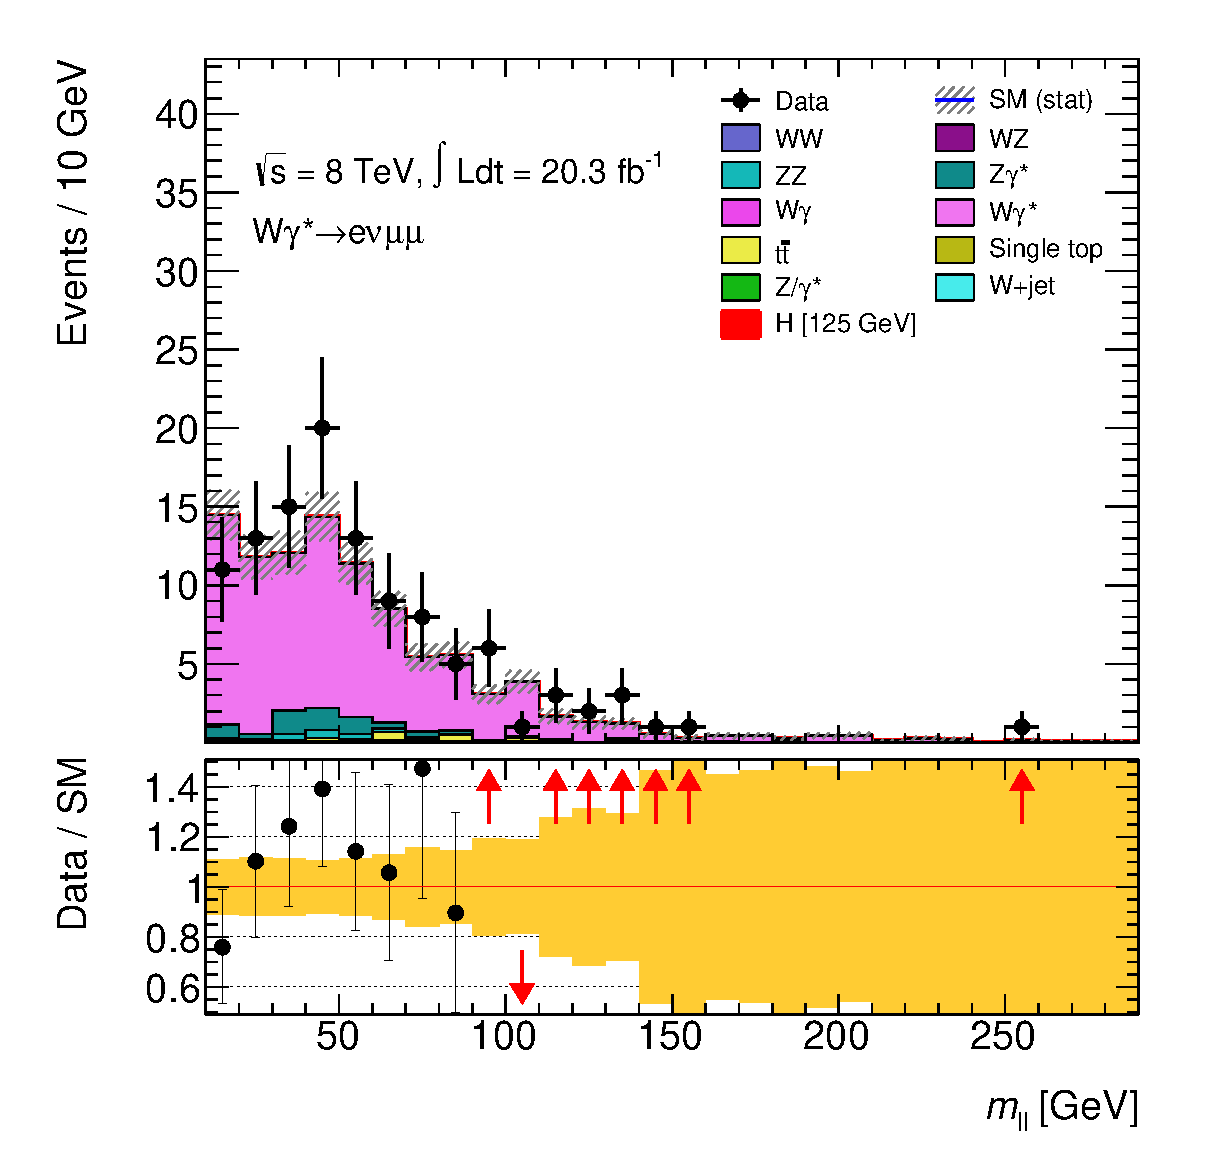
\includegraphics[width=0.48\textwidth]{tex/backgrounds/Wgstar/em_CutDPhiMax_Mll_mh125_lin}
	\\
	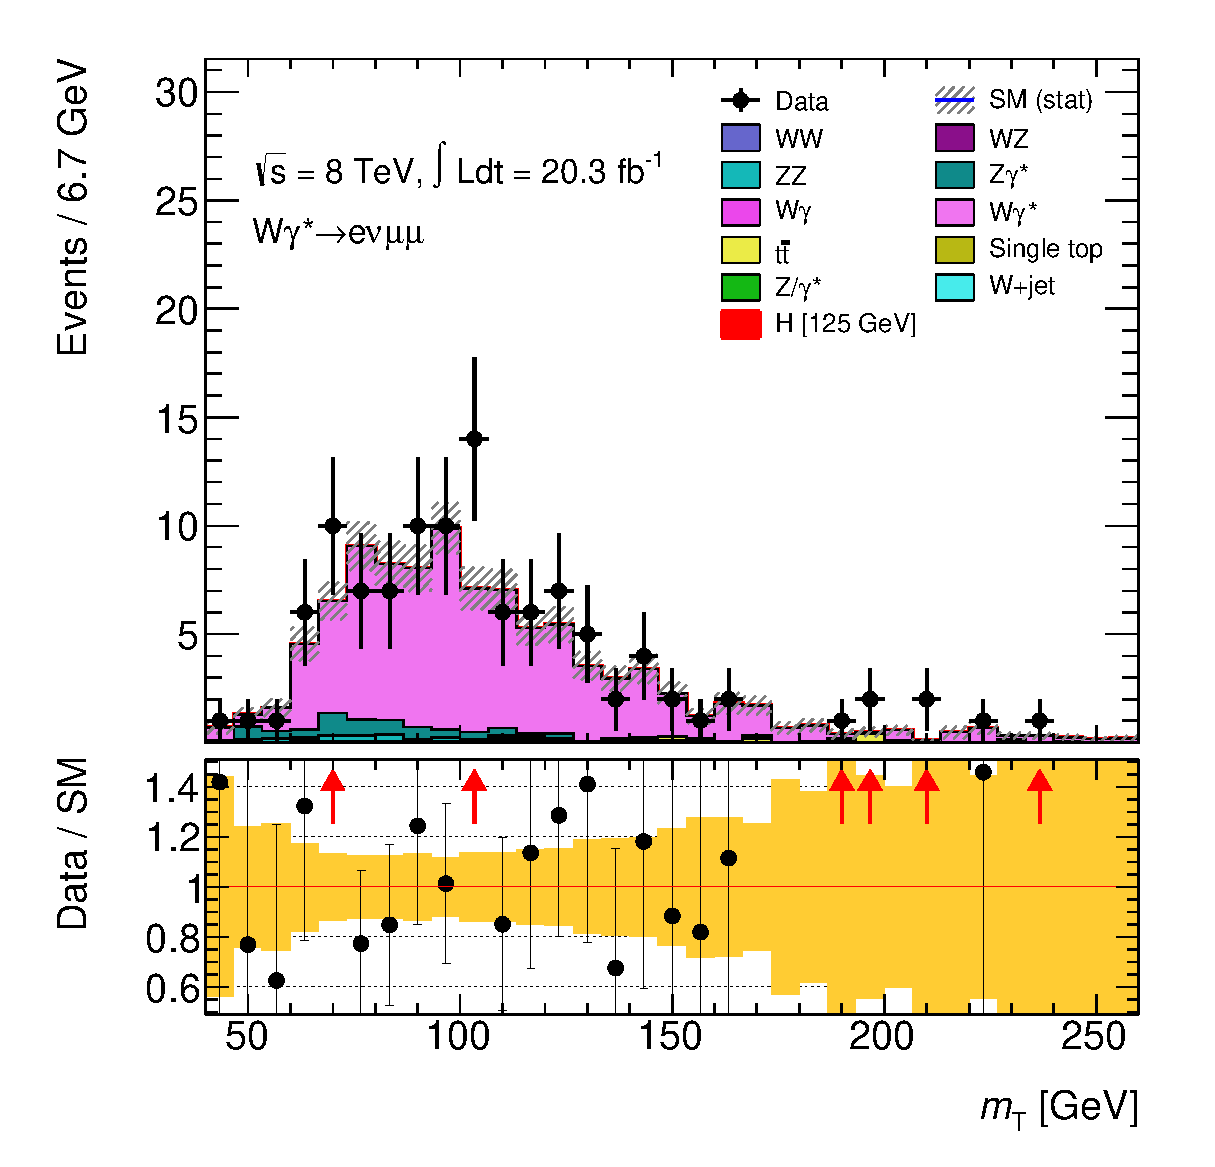
\includegraphics[width=0.48\textwidth]{tex/backgrounds/Wgstar/em_CutDPhiMax_MT_TrackHWW_Clj_mh125_lin}
	\hfill
	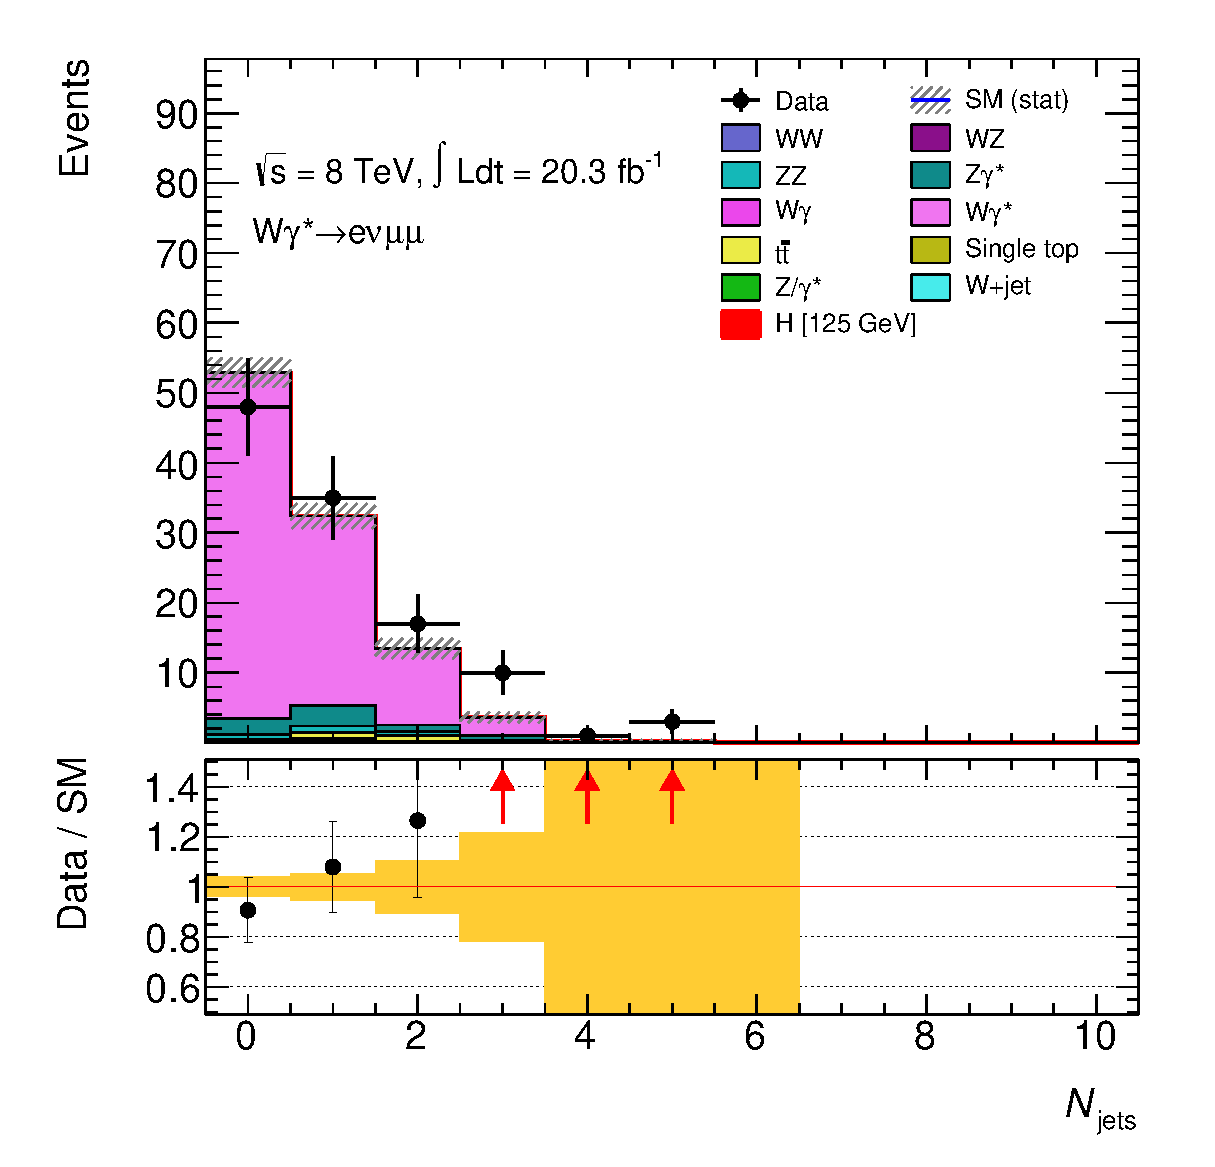
\includegraphics[width=0.48\textwidth]{tex/backgrounds/Wgstar/em_CutDPhiMax_m_jet_n_mh125_lin}
	\caption{The \ptsubleadlep (top left), \mll (top right), \mt (bottom left) and \njets 
	(bottom right) distributions in the \Wgstar validation region. Leptonic observables are 
	defined with the electron and the leading muon.}
	\label{fig:wgstar:vr}
\end{figure}

It should be noted that the \Wgstar VR does not test the modelling of 
\HepProcess{\Wgstar \HepTo \Plepton\Pnu\Pe\Pe}, which can contribute background events via 
an additional mechanism: both electrons can be reconstructed as a single electron when 
$\Delta R\parenths{\Pe,\Pe}$ is very small. However, the good agreement in the same-sign 
control region suggests that this is well modelled.



\subsection{\ZZ and \Zgstar}
\label{sec:diboson:zz}

Similar to \Section~\ref{sec:diboson:wgstar}, the \ZZ and \Zgstar processes share a 
\HepProcess{\Plepton\Plepton\Plepton'\Plepton'} final state, and are modelled together in 
order to include their interference. Again, the phase space is split: high mass 
``\ZZ'' events with \unit{$m_{\HepProcess{\Plepton\Plepton}} > 4$}{\GeV} and 
\unit{$m_{\HepProcess{\Plepton'\Plepton'}} > 4$}{\GeV}, and low mass ``\Zgstar'' events 
with \unit{$m_{\HepProcess{\Plepton\Plepton}} > 4$}{\GeV} and 
\unit{$m_{\HepProcess{\Plepton'\Plepton'}} < 4$}{\GeV}.\footnote{
	It is these ``\ZZ'' and ``\Zgstar''	MC samples that are referred to as the \ZZ and 
	\Zgstar backgrounds, though each sample contains both the \ZZ and \Zgstar processes.
}
The corresponding ``\HepProcess{\Pgammastar\Pgammastar}'' process is not modelled due to 
technical limitations. In ambiguous cases ($\Plepton = \Plepton'$), the lowest mass 
opposite-sign same-flavour dilepton pair is used to split the phase space.

\ZZ is modelled at NLO by \meps{\powhegbox}{\pythia{8}} and the NNLO \ggZZ diagrams are 
also modelled by \meps{\ggtozz}{\fherwig}. \Zgstar is modelled by \sherpa and is normalised 
to the NLO cross section calculated with \mcfm. As in \Section~\ref{sec:diboson:wgstar}, 
this $K$-factor is calculated at high $m_{\HepProcess{\Plepton'\Plepton'}}$ and 
extrapolated to low $m_{\HepProcess{\Plepton'\Plepton'}}$.

Neither background contributes significantly to the signal region. However, it is important 
to model the \Zgstar background in the \Zgamma validation region (see 
\Section~\ref{sec:diboson:wgamma}) and when measuring the \Zjets fake factor (see 
\Section~\ref{sec:wjets:zjet_ff}).

